\section{Hiệu năng thuật toán}
Trong phần này chúng ta sẽ xem xét hiệu năng của ALNS. Để thấy rõ sự khác biệt, các đồ thị được trình bày dưới đây là kết quả cho cấu hình $1000$ yêu cầu. Ngoài ra, để tránh dài dòng, các đồ thị được thể hiện cho 3 cầu hình C1\_10\_1, R1\_10\_1, RC1\_10\_1. Hiệu năng của các thuật toán đối với các cấu hình khác là tương tự. Chúng ta sẽ so sánh hiệu năng của ALNS nguyên bản, B-ALNS và một framework rất nổi tiếng trong cộng đồng là \code{Google OR-Tools}. Hiệu năng được so sánh cho cả phiên bản đơn luồng và đa luồng của ALNS.

\subsection{Giá trị hàm mục tiêu}

Trước hết, giá trị hàm mục tiêu theo thời gian được xem xét. Các đồ thị dưới đây cho thấy giá trị hàm mục tiêu theo thời gian khi chạy thuật toán với thời gian chạy 60 giây và được phóng đại để nhìn rõ hơn sự khác biệt trong 10 giây đầu tiên. Đồ thị được chia làm 3 phần tương ứng với 3 cấu hình khác nhau.

\begin{figure}[H] % places figure environment here   
  \label{fig:perf_ct_c1}
  \begin{subfigure}{.5\textwidth}
    \centering
    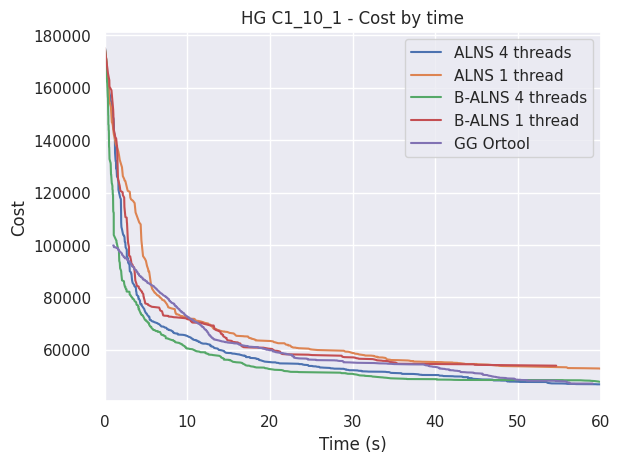
\includegraphics[width=1\linewidth]{figures/cost_time_60s_C1_10_1.png}
    \caption{60s}
    \label{fig:perf_ct_c1_60s}
  \end{subfigure}%
  \begin{subfigure}{.5\textwidth}
    \centering
    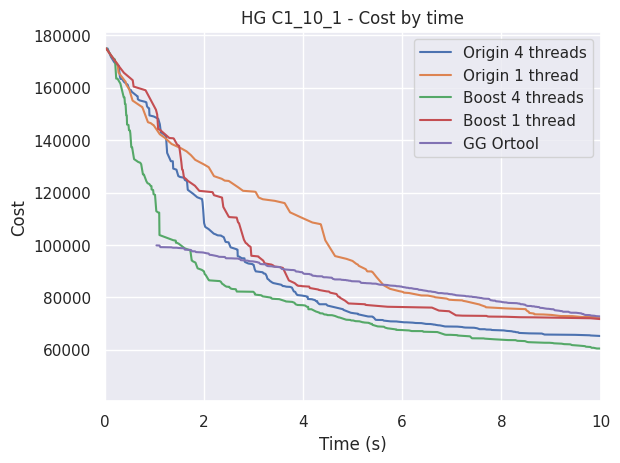
\includegraphics[width=1\linewidth]{figures/cost_time_10s_C1_10_1.png}
    \caption{10s}
    \label{fig:perf_ct_c1_10s}
  \end{subfigure}
  \caption{Giá trị hàm mục tiêu theo thời gian, cấu hình C1\_10\_1}
\end{figure}

\begin{figure}[H] % places figure environment here   
  \label{fig:perf_ct_r1}
  \begin{subfigure}{.5\textwidth}
    \centering
    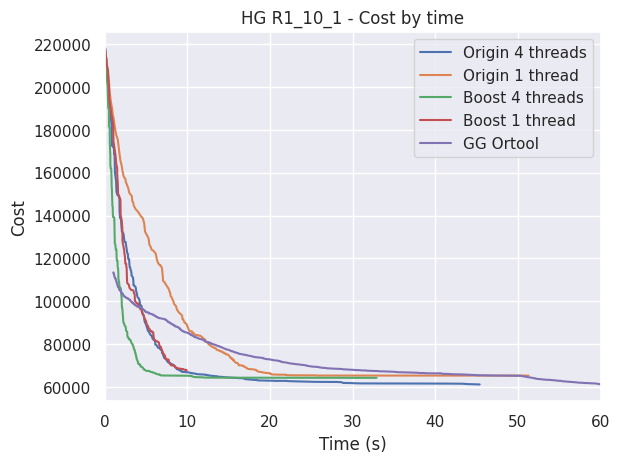
\includegraphics[width=1\linewidth]{figures/cost_time_60s_R1_10_1.png}
    \caption{60s}
    \label{fig:perf_ct_r1_60s}
  \end{subfigure}%
  \begin{subfigure}{.5\textwidth}
    \centering
    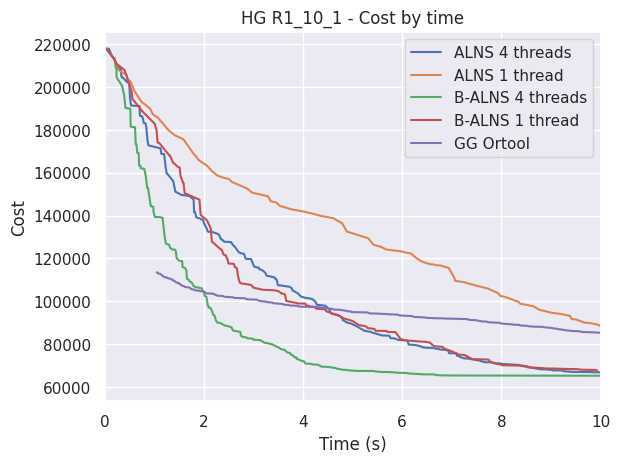
\includegraphics[width=1\linewidth]{figures/cost_time_10s_R1_10_1.png}
    \caption{10s}
    \label{fig:perf_ct_r1_10s}
  \end{subfigure}
  \caption{Giá trị hàm mục tiêu theo thời gian, cấu hình R1\_10\_1}
\end{figure}

\begin{figure}[H] % places figure environment here   
  \label{fig:perf_ct_r1}
  \begin{subfigure}{.5\textwidth}
    \centering
    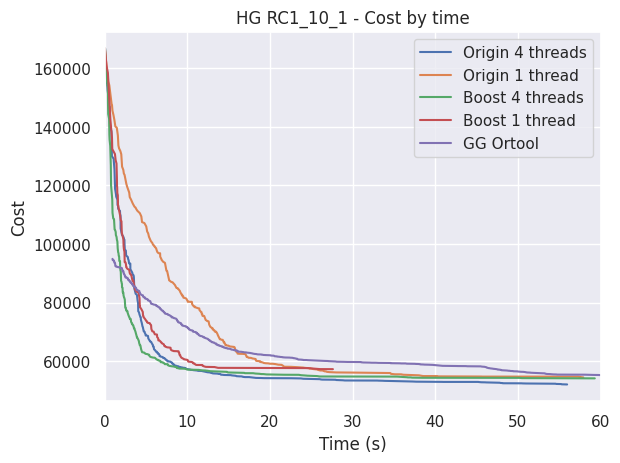
\includegraphics[width=1\linewidth]{figures/cost_time_60s_RC1_10_1.png}
    \caption{60s}
    \label{fig:perf_ct_r1_60s}
  \end{subfigure}%
  \begin{subfigure}{.5\textwidth}
    \centering
    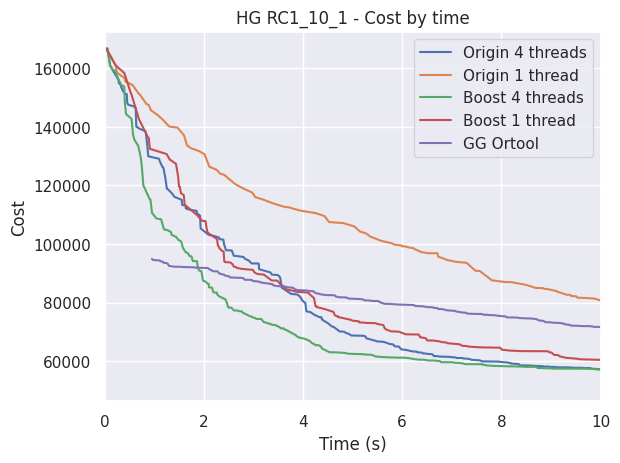
\includegraphics[width=1\linewidth]{figures/cost_time_10s_RC1_10_1.png}
    \caption{10s}
    \label{fig:perf_ct_r1_10s}
  \end{subfigure}
  \caption{Giá trị hàm mục tiêu theo thời gian, cấu hình RC1\_10\_1}
\end{figure}

Với thời gian chạy lâu, các thuật toán đều chững lại bởi khi đó các tuyến đường đã khá chật chội, việc "sửa chữa" là khó khăn hơn giai đoạn đầu rất nhiều. Nói cách khác, thuật toán bị bẫy trong nghiệm tối ưu cục bộ. Khi chạy thuật toán với thời gian lâu hơn (timeout 10 phút), tác giả nhận thấy hàm mục tiêu không giảm đáng kể nữa. Chính vì thế, thời gian chạy 60 giây được lựa chọn để vừa phù hợp với thực tế và tránh việc chạy quá lâu.

Ta thấy một xu hướng rõ ràng, trong giai đoạn đầu, B-ALNS tăng tốc hiệu năng của ALNS một cách đáng kể. Với thời gian chạy dưới 10 giây, B-ALNS đơn luồng cho hiệu năng gần như tương đương với ALNS với 4 luồng. Nghĩa là, B-ALNS tiết kiệm khoảng $75\%$ tài nguyên CPU để đạt kết quả tương đương với ALNS trong thời gian chạy dưới 10 giây. Chưa kể, memory cũng được tiết kiệm một cách đáng kể khi B-ALNS sử dụng 1 luồng thay vì 4 luồng. Khi so sánh với ALNS đơn luồng, B-ALNS đơn luồng cho hiệu năng vượt trội. Điều này cho thấy, B-ALNS có thể được sử dụng để giải quyết các bài toán lớn với tài nguyên hạn chế. 

Khi nâng số luồng của B-ALNS lên bằng với số luồng của ALNS, ta thấy rằng, hàm mục tiêu giảm nhanh hơn trong giai đoạn dầu. Đặc biệt trong các cấu hình mà địa điểm của yêu cầu có độ ngẫu nhiên cao (lớp R và RC), B-ALNS cho hiệu năng rất tốt. 

Khi so sánh với \code{Google OR-Tools}, ta thấy rằng, \code{Google OR-Tools} cho hiệu năng tốt trong thời gian chạy từ 2 đến 4 giây đầy tiên. Tuy nhiên với thời gian chạy dưới 1 giây, \code{Google OR-Tools} không thể cho ra kết quả. Với thời gian chạy lâu hơn, \code{Google OR-Tools} cho hiệu năng không tốt bằng ALNS hay B-ALNS. 

Như vậy đối với các nghiệp vụ yêu cầu một kết quả tốt trong thời gian ngắn, B-ALNS là lựa chọn tốt nhất. Khi tiến hành đo đạc với thời gian chạy dài (timeout lớn hơn 1 phút), tác giả nhận thấy rằng, ALNS là tốt nhất trong các thuật toán được đề cập ở đây. Các kết quả được chỉ ra trong phần trước là giá trị hàm mục tiêu khi sử dụng ALNS nguyên bản.

\subsection{Số xe}

Chúng ta cũng nhận thấy một xu hướng tương tự như khi so sánh hiệu năng của các thuật toán khi sử dụng độ đo là giá trị hàm mục tiêu. B-ALNS cho hiệu năng vượt trội trong giai đoạn đầu. B-ALNS đơn luồng cho hiệu năng tương đương với ALNS với 4 luồng. Với cấu hình lớp R, B-ALNS tiết kiệm được khoảng $30\%$ số xe so với ALNS trong thời gian chạy từ 2 tới 4 giây! Việc tiết kiệm hàng trăm xe có ý nghĩa rất lớn trong thực tế. Thường thì chi phí cho một xe (thuê, hoặc mua, nhiên liệu, chi phí cho tài xế, ...) là rất lớn. Việc tiết kiệm số xe sẽ giúp giảm chi phí vận hành của doanh nghiệp một cách đáng kể. 

Với thời gian chạy lâu hơn, đương nhiên chúng ta rất khó để giảm được số xe nữa, vì hầu hết các tuyến đường đến lúc này đã chật chội hơn đáng kể so với giai đoạn đầu.

\begin{figure}[H] % places figure environment here   
  \label{fig:perf_ct_c1}
  \begin{subfigure}{.5\textwidth}
    \centering
    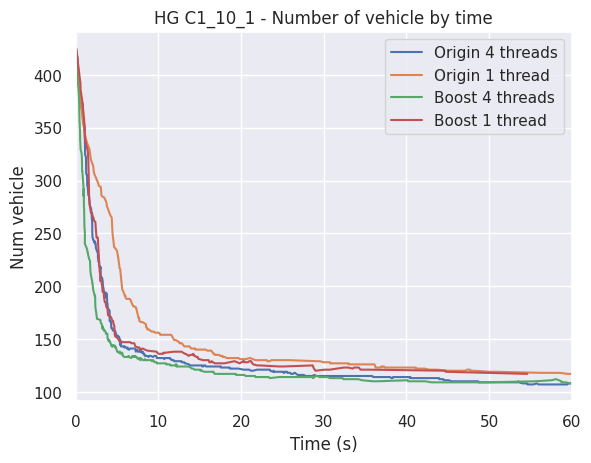
\includegraphics[width=1\linewidth]{figures/nv_time_60s_C1_10_1.png}
    \caption{60s}
    \label{fig:perf_ct_c1_60s}
  \end{subfigure}%
  \begin{subfigure}{.5\textwidth}
    \centering
    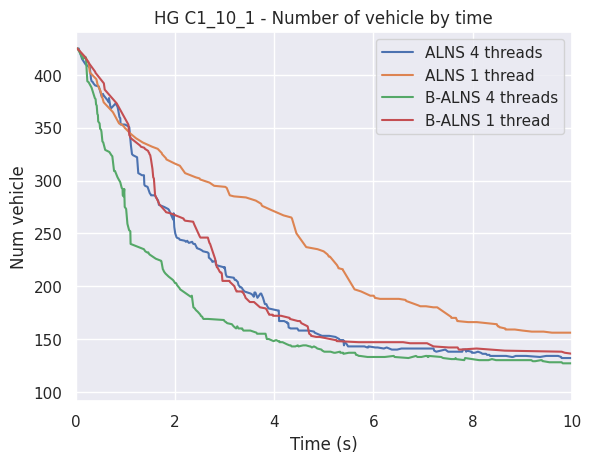
\includegraphics[width=1\linewidth]{figures/nv_time_10s_C1_10_1.png}
    \caption{10s}
    \label{fig:perf_ct_c1_10s}
  \end{subfigure}
  \caption{Số xe sử dụng theo thời gian, cấu hình C1\_10\_1}
\end{figure}

\begin{figure}[H] % places figure environment here   
  \label{fig:perf_ct_r1}
  \begin{subfigure}{.5\textwidth}
    \centering
    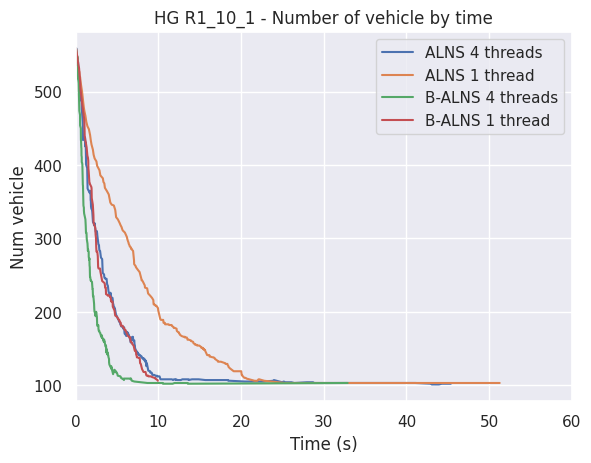
\includegraphics[width=1\linewidth]{figures/nv_time_60s_R1_10_1.png}
    \caption{60s}
    \label{fig:perf_ct_r1_60s}
  \end{subfigure}%
  \begin{subfigure}{.5\textwidth}
    \centering
    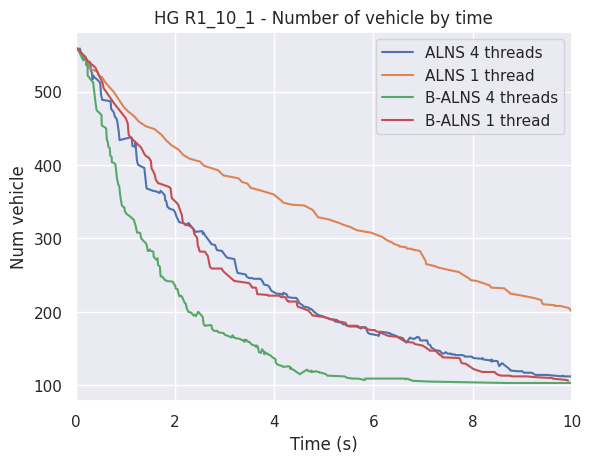
\includegraphics[width=1\linewidth]{figures/nv_time_10s_R1_10_1.png}
    \caption{10s}
    \label{fig:perf_ct_r1_10s}
  \end{subfigure}
  \caption{Số xe sử dụng theo thời gian, cấu hình R1\_10\_1}
\end{figure}

\begin{figure}[H] % places figure environment here   
  \label{fig:perf_ct_r1}
  \begin{subfigure}{.5\textwidth}
    \centering
    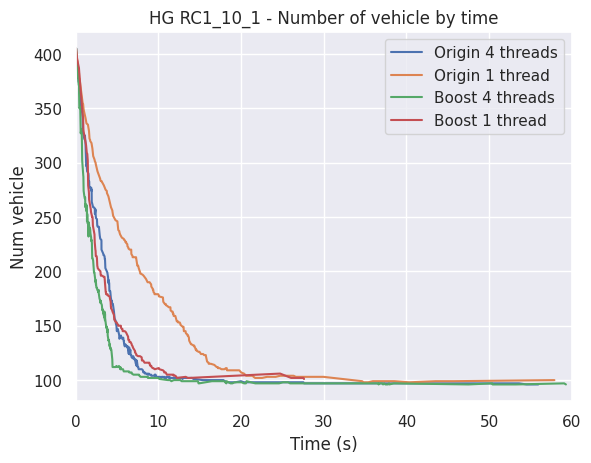
\includegraphics[width=1\linewidth]{figures/nv_time_60s_RC1_10_1.png}
    \caption{60s}
    \label{fig:perf_ct_r1_60s}
  \end{subfigure}%
  \begin{subfigure}{.5\textwidth}
    \centering
    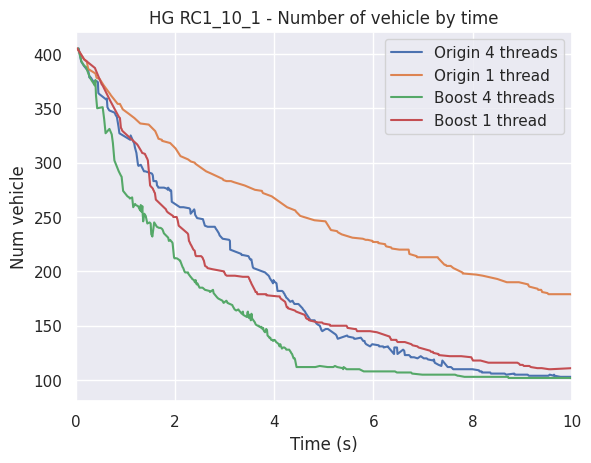
\includegraphics[width=1\linewidth]{figures/nv_time_10s_RC1_10_1.png}
    \caption{10s}
    \label{fig:perf_ct_r1_10s}
  \end{subfigure}
  \caption{Số xe sử dụng theo thời gian, cấu hình RC1\_10\_1}
\end{figure}